
\documentclass[11pt]{article}

\usepackage{fullpage,epsfig,latexsym,picinpar,amsbsy,amsmath,algorithm}
\usepackage[noend]{algpseudocode}
\usepackage{xspace}


\setlength{\evensidemargin}{0.1in}
\setlength{\oddsidemargin}{0.1in}
\setlength{\textwidth}{6.6in}
\setlength{\topmargin}{0.0in}
\setlength{\textheight}{8.7in}
\setlength{\headheight}{0in}
\setlength{\headsep}{0in}
\setlength{\topsep}{0in}
\setlength{\itemsep}{0in}
\renewcommand{\baselinestretch}{1.1}
\parskip=0.080in
                                                                                                                         
\newcommand{\parend}[1]{{\left( #1  \right) }}
\newcommand{\spparend}[1]{{\left(\, #1  \,\right) }}
\newcommand{\angled}[1]{{\left\langle #1  \right\rangle }}
\newcommand{\brackd}[1]{{\left[ #1  \right] }}
\newcommand{\spbrackd}[1]{{\left[\, #1  \,\right] }}
\newcommand{\braced}[1]{{\left\{ #1  \right\} }}
\newcommand{\leftbraced}[1]{{\left\{ #1  \right. }}
\newcommand{\floor}[1]{{\left\lfloor #1\right\rfloor}}
\newcommand{\ceiling}[1]{{\left\lceil #1\right\rceil}}
\newcommand{\barred}[1]{{\left|#1\right|}}
\newcommand{\doublebarred}[1]{{\left|\left|#1\right|\right|}}
\newcommand{\spaced}[1]{{\, #1\, }}
\newcommand{\suchthat}{{\spaced{|}}}
\newcommand{\numof}{{\sharp}}
\newcommand{\assign}{{\,\leftarrow\,}}
                                                                                                                         
\newcommand{\veps}{{\varepsilon}}
\newcommand{\Sigmastar}{{\Sigma^\ast}}
\newcommand{\barx}{{ \bar x}}

\newcommand{\half}{{\mbox{$\frac{1}{2}$}}}
\newcommand{\threehalfs}{{\mbox{$\frac{3}{2}$}}}





\usepackage{listings}
\usepackage{color}

\definecolor{dkgreen}{rgb}{0,0.6,0}
\definecolor{gray}{rgb}{0.5,0.5,0.5}
\definecolor{mauve}{rgb}{0.58,0,0.82}

\lstset{frame=tb,
  language=Java,
  aboveskip=3mm,
  belowskip=3mm,
  showstringspaces=false,
  columns=flexible,
  basicstyle={\small\ttfamily},
  numbers=none,
  numberstyle=\tiny\color{gray},
  keywordstyle=\color{blue},
  commentstyle=\color{dkgreen},
  stringstyle=\color{mauve},
  breaklines=true,
  breakatwhitespace=true,
  tabsize=3
}

\begin{document}

\centerline{\large \bf CS235 ASSIGNMENT}
\centerline{Yidi Wang}
\centerline{862114701}

\vskip 0.1in

%%%%%%%%%%%%%%%%%%%%%%%%%%%%

\paragraph{Question 1}\mbox{} \\
\noindent
\textbf{Part 1}
\begin{verbatim}
clear; clc;
edgelist = dlmread('graph.txt');
edgelist = unique(edgelist, 'rows');
A = sparse(edgelist(:,1), edgelist(:,2), 1);
\end{verbatim}

\noindent
\textbf{Part 2, 3} \\
Three dense blocks are annotated by red circles.
\begin{figure}[!h]
    \centering
    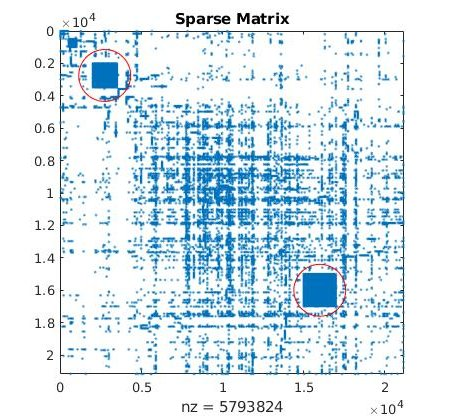
\includegraphics[width=\linewidth]{figs/q1.jpg}
    \caption{spy-plot}
    \label{fig::spy}
\end{figure}

%%%%%%%%%%%%%%%%%%%%%%%%%%%%
\paragraph{Question 2}\mbox{} \\
\noindent
\textbf{Part 1} \\
The number of connected nodes are calculated for each node in the edge-list of the graph.
\begin{verbatim}
max_node = max(edgelist(:));
deg_node = zeros(1, max_node);
for i = 1:max_node
    deg_node(i) = sum(rows(:) == i);
end
\end{verbatim}

\noindent
\textbf{Part 2} \\
\begin{figure}[!h]
    \centering
    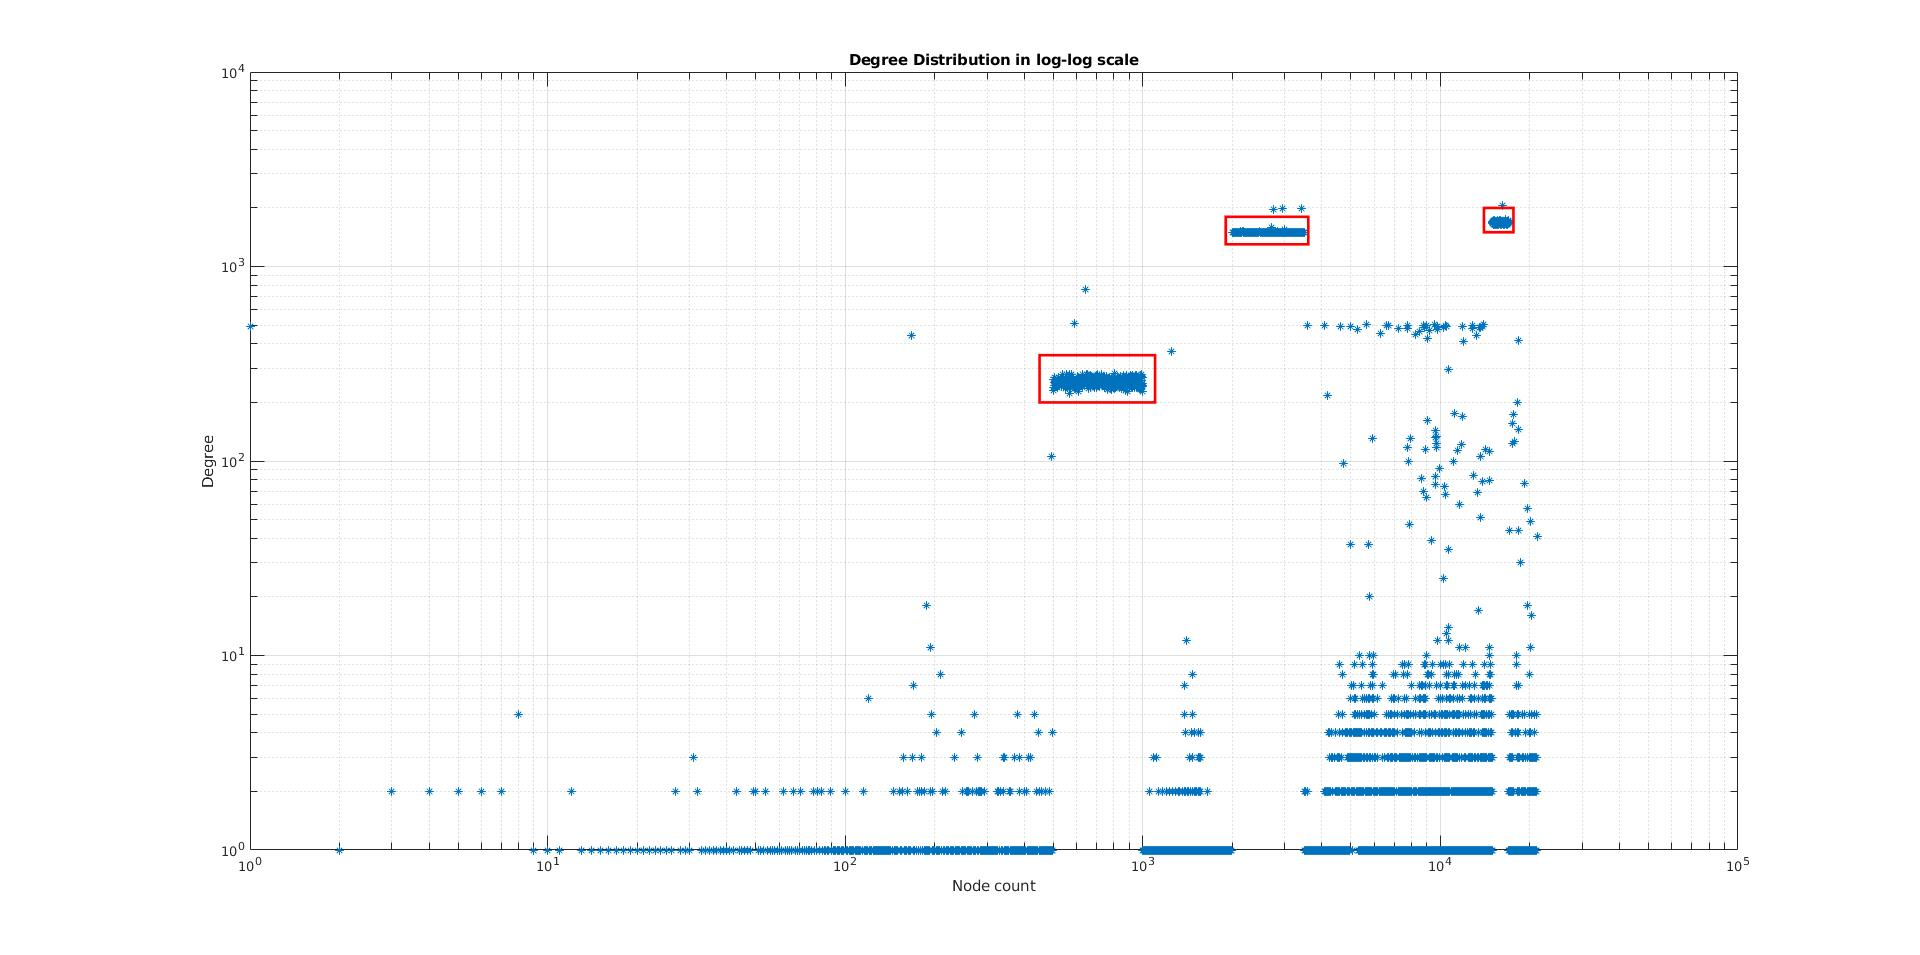
\includegraphics[width=\linewidth]{figs/q2.jpg}
    \caption{Degree distribution in log-log scale}
    \label{fig::deg_log}
\end{figure}

\noindent
\textbf{Part 3} \\
Yes. In the clean degree distribution figure, the majority of the nodes have a small degree. While the degree becomes larger, the number of corresponding nodes become less and less. Degree and node counts are negtively correlated. However, in this distribution, node count is increasing while the degree increase. They are positively correlated.

\noindent
\textbf{Part 4} \\
(a). There are three abnormal blocks. They are annotated in red circles. Above the $10^2$ on the y axis in the above figure (when degree is big enough), there are three nearly horizontal lines, which means that there are many consecutive nodes having similar degrees. This will cause dense blocks in the sparse matrix.
\noindent
(b). The upper thick line area in Fig.\ref{fig::deg_log} is corresponding to the upper right dense block in Fig.\ref{fig::spy}. The lower left thick line in Fig.\ref{fig::deg_log} is corresponding to the lowest right dense block in Fig.\ref{fig::spy}. And the middle thick line in Fig.\ref{fig::deg_log} is corresponding to the middle block in Fig.\ref{fig::spy}.

\paragraph{Question 3}\mbox{} \\
\noindent
\textbf{Part 1} \\


\noindent
\textbf{Part 2} \\
(a). % TODO: compute square error
\begin{verbatim}
[u,s,v] = svds(A);
ds = diag(s);
dsp = norm(ds(n+1:end)) / norm(ds);
\end{verbatim}
I tried the above code with different $n$. When $n = 2$, the error is $0.1157$. When $n = 3$, the error is $0.0271$. So, if we want a reconstruction correctness larger than $90\%$, the number of singular value is 3.
$$
\begin{bmatrix} 
    1679.9  \\
    1501.0  \\ 
    255.22  \\
    37.715  \\
    35.5439
\end{bmatrix}
$$

\noindent
(b). 
\begin{figure}[!h]
    \centering
    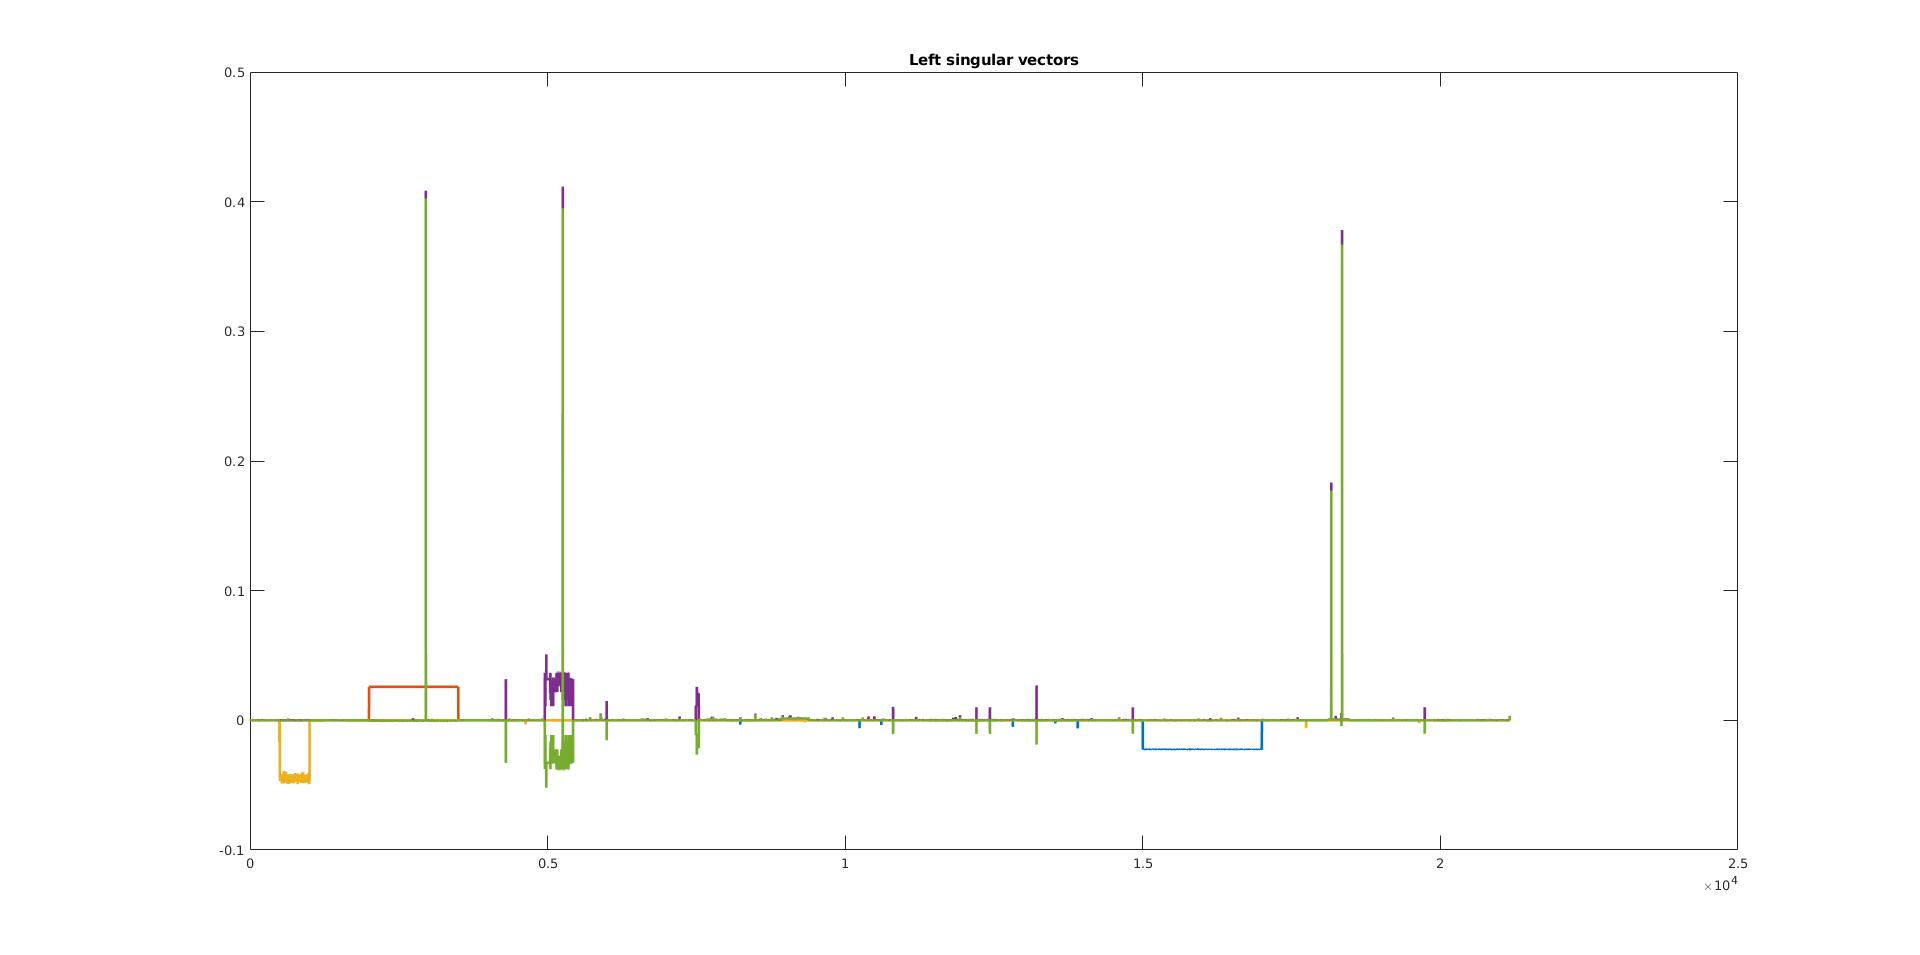
\includegraphics[width=\linewidth]{figs/q3.jpg}
    \caption{Left singular vectors}
    \label{fig::vec}
\end{figure}

\noindent
(c). We can identify from Fig.\ref{fig::vec} that there are three abnormal blocks in the sparse matrix. The first two left singular vectors' range are much bigger than the last three vectors. Let's explain it from the geometric meaning of SVD decomposition: $S$ means the scale transformation of the original matrix, while $U$ means the rotation to the matrix. 


\end{document}

